%% PNAStwoS.tex
%% Sample file to use for PNAS articles prepared in LaTeX
%% For two column PNAS articles
%% Version: Apr 15, 2008


%% BASIC CLASS FILE
%\documentclass{pnastwo}
\documentclass[10pt]{article}
\usepackage[hang,flushmargin]{footmisc}
\usepackage{mathtools}
\usepackage{capt-of}
\usepackage{xcolor}
%% ADDITIONAL OPTIONAL STYLE FILES
\usepackage{mathptmx}
\usepackage{graphicx}
\usepackage[margin=1in]{geometry}
\usepackage[numbers]{natbib}
%\newcommand{\rom}[1]{\uppercase\expandafter{\romannumeral #1\relax}}%\usepackage{titlesec}
%\usepackage[pdftex]{graphicx}
%\usepactxkage{pnastwoF}
\usepackage{amssymb,amsfonts,amsmath}
%\usepackage[numbers,sort&compress]{natbib}
\usepackage{mhchem}
%\usepackage{subeqnarray}
%\usepackage{cases}
\usepackage{color}
\usepackage{verbatim}
\usepackage{xcolor}
%\usepackage{romannum}
\usepackage{braket}
\usepackage{siunitx}
\usepackage{tocloft}
\usepackage{units}
\usepackage{array}
\usepackage{longtable}
\usepackage{hyperref}
\usepackage{tabularx}
\usepackage{multirow}
\usepackage[skins,theorems]{tcolorbox}
\tcbset{highlight math style={enhanced,
  colframe=red,colback=white,arc=0pt,boxrule=1pt}}
\renewcommand\thesection{\arabic{section}}
%\usepackage[figurename=Figure.,
%                  justification=RaggedRight,
%                  labelfont={bf, footnotesize},
%                  textfont={footnotesize},position=top]{caption}
\usepackage{array}
\usepackage{longtable}
\usepackage{tabularx}
\usepackage{multirow}
\usepackage{fixltx2e}
\usepackage{textgreek}
\usepackage[T1]{fontenc}
%\usepackage{ulem}
\usepackage[normalem]{ulem} %to strike the words
\newcolumntype{C}[1]{>{\arraybackslash}p{#1}}
\usepackage[labelfont=bf]{caption}


\usepackage{color} %for \textcolor
\usepackage{epsfig}
\usepackage{floatflt}
\usepackage{wrapfig}
%\usepackage{titlesec}


\usepackage{float}
\usepackage{times}
\usepackage{helvet}
\usepackage{amsmath}
\headheight = 0.0 in
\headsep = 0.0 in

\newcommand{\todo}[1]{{\color{red}{[#1]}}}
\renewcommand{\thefootnote}{\fnsymbol{footnote}}
%\renewcommand{\thesection}{\Alph{section}}
\renewcommand{\familydefault}{\sfdefault}

\setcounter{secnumdepth}{5}
\setcounter{tocdepth}{5}


\long\def\symbolfootnote[#1]#2{\begingroup%
\def\thefootnote{\fnsymbol{footnote}}\footnote[#1]{#2}\endgroup}

\renewcommand{\figurename}{{Fig.}}

\newcommand{\ra}{\rightarrow}
\newcommand{\nubot}{nubot}
\newcommand{\degree}{$^{\circ}$C}

\long\def\remove #1{}

\newcommand{\red}[1]{\textcolor{red}{#1}}
\newcommand{\redd}[1]{\textcolor{red}{#1}}
\newcommand{\peng}[1]{\textcolor{red}{peng: #1}}
\newcommand{\tbd}[1]{\textcolor{red}{To be added: #1}}


%\setcounter{page}{1} \pagenumbering{arabic}
\pagestyle{plain} \setcounter{page}{1} \pagenumbering{arabic}

%\renewcommand{\theequation}{S\arabic{equation}}
%\renewcommand{\figurename}{\textbf{Supplemental Figure}}
%\renewcommand{\tablename}{\textbf{Supplemental Table}}
%\renewcommand{\thefigure}{S\arabic{figure}}
%\renewcommand{\thetable}{S\arabic{table}}
%\usepackage{helvet}
\renewcommand{\familydefault}{\sfdefault}
%\usepackage[T1]{fontenc}
%\usepackage{fourier}
%\usepackage{cmbright}
%\usepackage{etoolbox}
%\patchcmd{\thebibliography}{\section*{\refname}}{}{}{}
\renewcommand\refname{}
%\textcolor{black}{}
%\newcommand{\blackt}[1]{\textcolor{black}{#1}}
%\newcommand{\blue}[1]{\textcolor{red}{#1}}
\newcommand{\sub}[1]{\textsubscript{#1}}
\newcommand{\supp}[1]{\textsuperscript{#1}}
\renewcommand{\thefootnote}{$\dagger$}
\newcommand{\redt}[1]{\textcolor{black}{#1}}
\newcommand{\aeb}[1]{\textcolor{black}{#1}}
\newcommand{\aebN}[1]{\textcolor{black}{#1}}
\newcommand{\orangecl}[1]{\textcolor{black}{#1}}
\newcommand{\clred}[1]{\textcolor{red}{#1}}
\newcommand{\clblue}[1]{\textcolor{blue}{#1}}
\newcommand{\clredd}[1]{\textcolor{black}{#1}}
\newcommand{\clredtable}[1]{\color{black}{#1}}
\newcommand{\tsub}[1]{\textsubscript{#1}}
\newcommand{\tsup}[1]{\textsuperscript{#1}}
 \renewcommand{\familydefault}{\sfdefault}

\DeclareSIUnit{\molar}{M}
\DeclareSIUnit{\nucl}{nucl.}
\DeclareSIUnit{\aa}{aa}

%\newcommand{\supp}[1]{\supp{#1}}
%\usepackage{mathpazo}
%% OPTIONAL MACRO DEFINITIONS
%\def\s{\sigma}
\usepackage[
singlelinecheck=true % <-- important
]{caption}

\makeatletter
\renewcommand\paragraph{\@startsection{paragraph}{4}{\z@}%
            {-2.5ex\@plus -1ex \@minus -.25ex}%
            {1.25ex \@plus .25ex}%
            {\small\small\bfseries}}
\makeatother
\setcounter{secnumdepth}{4} % how many sectioning levels to assign numbers to
\setcounter{tocdepth}{4}    % how many sectioning levels to show in ToC
%\usepackage[sort, numbers]{natbib}
%\setcitestyle{square}
%\setcounter{secnumdepth}{4}

%\titleformat{\paragraph}
%{\normalfont\normalsize\bfseries}{\theparagraph}{1em}{}
%\titlespacing*{\paragraph}
%{0pt}{3.25ex plus 1ex minus .2ex}{1.5ex plus .2ex}

\renewcommand{\contentsname}{}
\renewcommand*\subsectionmark[1]{\markright{#1}}
\renewcommand{\thesubsection}{\arabic{subsection}}


\begin{document}

\title{Integrative Modeling of Bacterial H2O2 Stress Responses}
\author{Chen Liao}

\maketitle
\tableofcontents

%\begin{abstract}
%The abstract text goes here.
%\end{abstract}

\clearpage
\section{Background knowledge}

Reactive oxygen species (ROS) such as superoxide, hydrogen peroxide (H2O2), and hydroxyl radical, can be produced by intracellular aerobic respiration and/or environments. They are toxic to bacterial cells, leading to loss of fitness, including high mutation rates, growth defects, and even cell death. Biochemically, there are two basic classes of H2O2-degrading proteins
\begin{enumerate}
\centering
\item{Catalase: $2H_2O_2 \rightarrow O_2+2H_2O$}
\item{Peroxidases: $RH_2+H_2O_2 \rightarrow R+2H_2O$}
\end{enumerate}
The electron source of catalase is from H2O2 itself and no exogenous electron source is needed. However, peroxidases can differ in their electron donors (i.e., $RH_2$), which could be glutathione, thioredoxins, NAD(P)H, cytochrome \textit{c}, dyes and other unknowns. 

Catalases rely on iron or manganese so they fall into two categories: heme (an iron-containing compound) calatases and non-heme catalases (or manganese). Catalases with only catalatic activity are called mono-functional catalases, and those with both catalatic activity and peroxidatic activities are referred to as bifunctional catalases or catalase-peroxidases.

Peroxidases also fall into two categories: thiol (i.e., RSH)-based peroxidases (peroxiredoxins; abbr. Prx) and non-thiol peroxidases. All peroxiredoxins contain a conserved cysteine that reacts with H2O2 and forms a disulfide before getting reduced back to free thiol. Depending on the variations in the mechanisms of thiol regeneration, peroxidases can be further classified into four groups: alkylhydroperoxide reductases (AhpCF), thiol glutathione peroxidase (Tpx), bacterioferritin comigratory protein (BCP), and glutathione peroxidase (Gpx). 

GPx catalyzes the reaction of hydrogen peroxide with GSH to produce glutathione disulfide (GSSG). Glutathione disulfide is subsequently reduced through the actions of glutathione reductase and NADPH. 

H2O2 can also be eliminated by oxidizing the cysteine residues of intracellular proteins (Pr-SH=Pr-(SH)2). Cysteine (Cys) residues of intracellular proteins contain redox-sensitive thiols that are susceptible to oxidation. On oxidation, the Cys residues of proteins can be reduced, with different characteristics, depending on the
microenvironment, through a system of reactions involving GSH or Trx.

The thioredoxin-deficient mutant (trxA) was more sensitive to H2O2 than was the wild-type strain, when challenged in the stationary and exponentially growing phase. Thioredoxin reductase-deficient mutant (trxB) in the stationary phase also exhibited increased sensitivity, compared with the wild-type strain. These results indicated that reduced form of thioredoxin is required for defense against H2O2,

\subsection{\textit{Escherichia coli}}

Most of the following information about \textit{E. coli} antioxidant systems come from a review paper~\cite{mishra2012bacteria}. \textit{E. coli} has at least 9 enzymes that have been proposed to be calatases or peroxidases. The major H2O2 scavenging enzyme is Ahp (alkyl hydroperoxide reductase)~\cite{seaver2001alkyl}, which consists of two subunits: the small subunit (AhpC), which reduces organic peroxides to their corresponding alcohols, and the large subunit (AhpF), which is a close homologue of bacterial TrxR that can use either NADPH or NADH as a source of reducing power to reduce AhpC-disulfide. Even though AhpF can obtain electrons from NADH, based on the relatively low availability of NADH in cells, the AhpC is likely fueled predominantly by NADPH. When reducing power is limited (e.g., nutrient starvation), AhpCF has limited activity. 

\textit{E. coli} also contains two catalases, HPI (hydroperoxidase I, encoded by \textit{katG}) and HPII (hydroperoxidase II, encoded by \textit{katE}). Despite the key role of Ahp, catalase still has an important role in wild-type cells, because the activity of Ahp is saturated at a low concentration of H2O2 ($< 1~\mu M$). In contrast, catalases have high Km ($\sim 1~mM$), and therefore become the predominant scavenger when H2O2 concentrations are high. In contrast to Ahp, catalases can provide protection even in energy-depleted cells.

When the entry rate of H2O2 is high, basal level defense is inadequate and adaptive response is needed. Both Ahp and KatG are transcriptionally induced by the transcriptional regulator, OxyR~\cite{hillion2015thiol}. A key cysteine residue of the OxyR protein is oxidized by H2O2, triggering conformational change from an inactive form (i.e., reduced state) to an active form (oxidized state). The oxidized OxyR then binds to the promoter regions of many genes on the \textit{oxyR} regulon. Reduced OxyR is regenerated by the glutaredoxin/GSH/Gor system upon return to non-stress conditions.  

OxyR positively controls genes for peroxide detoxification, such as catalase and peroxiredoxin (katG, ahpCF), Fe-storage miniferritin (dps), glutaredoxin, thioredoxin and glutathione reductase (grxA, trxC, gor), sulfenic acid oxidoreductase (dsbG), ferric uptake regulator (fur), Fe-S-cluster assembly machinery (sufABCDE), ferrochelatase (hemH), manganese import (mntH) and the small RNA (oxyS)~\cite{hillion2015thiol}. OxyR negatively regulates its own expression and that of the genes for the ferric ion reductase (fhuF), the outer membrane protein (flu), the mannonate hydrolase (uxuAB) and gluconate permease (gntP)~\cite{hillion2015thiol}. A comprehensive list of genes in the \textit{oxyR} operon is available \href{https://ecocyc.org/gene?orgid=ECOLI\&id=EG10681\#tab=REGULON}{here}. 

Other catalases or peroxidases seem to be dispensible. KatE is induced at the transition from exponential phase to stationary phase by RpoS and its induction is OxyR-independent. Mutation in HPII did not affect the log-phase growth phenotype even in strains lacking HPI and/or Ahp~\cite{seaver2001alkyl}. Other peroxidases seem to play other functions than H2O2-degradation \textit{in vivo}, although their activity has been demonstrated. For example, the \textit{tpx} mutant did not show any phenotype under aerobic growth, while it is more sensitive to organic hydroperoxides. Deletion of \textit{btuE} (Gpx) also does not create sensitivity to H2O2, while the mutant is more sensitive to paraquat and tellurite~\cite{arenas2011escherichia}.

According to Masip et al.~\cite{masip2006many}, exponentially growing E. coli that lack GSH (gshA mutant) have normal resistance to H2O2, but when they reach stationary phase they are more susceptible to killing byH2O2 (9). E. coli gor mutants show diamide sensitivity similar
to gshA mutants, are somewhat sensitive to paraquat and cumene hydroperoxide, and show increased H2O2 sensitivity in a catalase mutant background. GSH also plays an indirect role in cells under peroxide stress by reducing oxidized OxyR by means of glutaredoxin 1.

The follwoing are based on~\cite{potamitou2002protein}. In a wild type strain, levels of Trx1 increased from the exponential to the stationary phase of growth (1.5-fold to 3400 ng/mg), as did levels of Grx2 (from 2500 to 8000 ng/mg). Grx3 and Trx2 levels were quite stable during growth (4500 and 200 ng/mg, respectively). Grx1 levels decreased from 600 ng/mg at the exponential phase to 285 ng/mg at the stationary phase. A large elevation of Grx1 (20–30-fold), was observed in null mutants for the thioredoxin system whereas levels of the other redoxins in all combinations of examined null mutants barely exceeded a 2–3-fold increase. Measurements of thymidine incorporation in newly synthesized DNA suggested that mainly Grx1 and, to a lesser extent, Trx1 contribute to the reduction of ribonucleotides. All glutaredoxin species were elevated in catalase-deficient strains, implying an antioxidant role for the glutaredoxins. Trx1, Trx2, and Grx1 levels increased after exposure to hydrogen peroxide and decreased after exposure to mercaptoethanol. The levels of Grx2 and Grx3 behaved exactly the opposite, suggesting that the transcription factor OxyR does not regulate their expression.

\subsection{\textit{Pseudomonas aeruginosa}}

KatA is the major catalase in \textit{P. aeruginosa} whose expression is constitutively highly in all phases of growth (high basal) but increased upon stationary growth phase and H2O2 treatment~\cite{heo2010major}. It is highly stable and can be found in the extracellular milieu, which ensures the survival of \textit{P. aeruginosa} cells in its biofilm state. Other typical antioxidant enzymes for the defense against H2O2 challenges include catalases (KatB and KatE) and alkyl hydroperoxide-reducing proteins (AhpB, AhpC, and Ohr). The \textit{katA}, \textit{katB}, \textit{ahpB}, and \textit{ahpCF} genes are positively regulated by OxyR. KatA was also found to be regulated by quorum sensing signals~\cite{hassett1999quorum} and stringent response~\cite{khakimova2013stringent}. Recently, it was reported that KatE was induced by high temperature and requires the disulfide bond formation system for its activity.

%%%%%%%%%%%%%%%%%%%%
%%%%%%%%%%%%%%%%%%%%
%%%%%%%%%%%%%%%%%%%%
\clearpage
\section{Modeling H2O2 diffusion, production and decomposition}

\subsection{Model assumptions}
The intracellular H2O2 concentration is determined by the balances of three processes: diffusion, production and decomposition (Fig.~\ref{fig:h2o2_decomposition_schematic_diagram}). To develop a model of H2O2 fluxes, the following assumptions are made
\begin{enumerate}
\item{Intracellular H2O2 is produced at a constant rate;}
\item{Two H2O2-degrading enzymes, Ahp and KatG, are considered;}
\item{Ahp becomes saturated at a low concentration of H2O2 (low $K_m$), while KatG has a high $K_m$. Therefore, decomposition of H2O2 by Ahp and KatG are modelled using Michaelis-Menten and first-order equation respectively;}
\item{The total OxyR concentration remains a constant and the equilibrium between oxidized and reduced forms of OxyR can be rapidly reached;}
\item{Both Ahp and KatG are regulated by the oxidized form of OxyR;}
\item{Both Ahp and KatG are stable proteins and not actively degraded.}
\end{enumerate}

\begin{figure}[h!]
\centering
  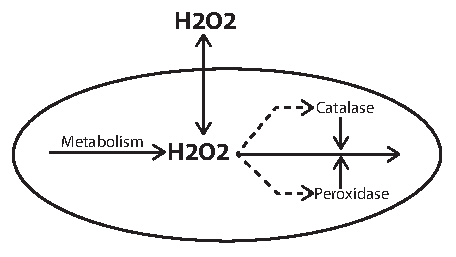
\includegraphics[width=0.5\linewidth]{h2o2_decomposition.pdf}
  \caption{Schematic diagram of H2O2 reactions. Gene expressions of catalases (KatG) and peroxidases (Ahp) are induced by H2O2 indirectly via oxidation of OxyR.}
  \label{fig:h2o2_decomposition_schematic_diagram}
\end{figure}

%%%%%%%%%%%%%%%%%%%%
\subsection{Mathematical equations}
Based on the above assumptions, the kinetic equations of intracellular ($[H_{i}]$) and extracellular ($[H_{o}]$) H2O2 concentrations are given by
\begin{eqnarray}
\frac{d[H_o]}{dt} &=& -\frac{([H_o]-[H_i])PA}{V_e} \\
\frac{d[H_i]}{dt} &=& \dfrac{k_{met}+([H_o]-[H_i])PA}{V_c} -k_{0,cat}[KatG][H_i] - \dfrac{k_{0,ahp}[Ahp][H_i]}{K_{m,ahp}+[H_i]}\label{eq:dhidt}
\end{eqnarray}
where $[KatG]$ and $[Ahp]$ are the concentrations of KatG and Ahp respectively. Parameters include the metabolic production rate of H2O2 ($k_{met}$), the membrane permeability ($P$), the surface area of the membrane ($A$), the cell volume ($V_c$), the medium volume ($V_e$), the specific activity of KatG ($k_{0,cat}$), the Ahp's turnover rate ($k_{0,ahp}$), and the half-maximal degradation concentration ($K_{m,ahp}$). 

Both glutaredoxin 1 and thioredoxin are able to reduce OxyR \textit{in vitro}; however, the former seems to predominate over the latter \textit{in vivo}~\cite{aaslund1999regulation}. The oxidized ($[OxyR_{ox}]$) and reduced ($[OxyR_{red}]$) forms of OxyR can be interconverted through two reactions
\begin{align*}
\ce{OxyR_{red} + n_{oxyr}H_2O_2 <->[k_{b+}][k_{b-}] OxyR_{red}(H_2O_2)_{n_{oxyr}} ->[k_{oxyr,ox}] OxyR_{ox}}
\end{align*}
\begin{align*}
\ce{OxyR_{red} + 4GSSG <->[k_{oxyr,ox1}][k_{oxyr,red1}] OxyR_{ox} + 8GSH }
\end{align*}
where $k_{b+}$ and $k_{b-}$ are the forward and reverse binding constants, $n_{oxyr}$ is the stoichiometry of H2O2 molecule in the binding complex between OxyR and H2O2, $k_{oxyr,ox}$ and $k_{oxyr,ox1}$ are the rates of H2O2- and GSH/GSSG ratio-dependent OxyR oxidation, and $k_{oxyr,red1}$ is the GSH/GSSG ratio-dependent OxyR reduction. Under the assumption of rapid binding/unbinding equilibrium between $OxyR_{red}$ and H2O2, the chemical kinetics in the equation can be described using differential-algebraic equations
\begin{eqnarray}
\frac{d[OxyR_{ox}]}{dt} &=& k_{switch}([H_i])[OxyR_{red}]+k_{oxyr,ox1}[OxyR_{red}][GSSG]^4-k_{oxyr,red1}[OxyR_{ox}][GSH]^8 \label{eq:doxyrox_dt} \\
k_{switch}([H_i]) &=& \frac{k_{oxyr,ox}[H_i]^{n_{oxyr}}}{K_{m,oxyr}^{n_{oxyr}}+[H_i]^{n_{oxyr}}} \label{eq:kswitch}\\
OxyR_t &=& [OxyR_{ox}]+[OxyR_{red}]
\end{eqnarray}
where $K_{m,oxyr}(=(k_{b-}+k_{oxyr,ox})/k_{b+})$ is the dissociation constant and $OxyR_t$ is the total OxyR concentration, which is assumed a constant. If we further assume that the equilibrium between $OxyR_{ox}$ and $OxyR_{red}$ can be rapidly reached and set Eq.~\ref{eq:doxyrox_dt} to zero, we obtain the fraction of oxidized OxyR at steady state
\begin{equation}\label{eq:doxyroxss_dt}
f_{oxyr}=\frac{[OxyR_{ox}]_{ss}}{OxyR_t} = \frac{k_{swtich}([H_i])+k_{oxyr,ox1}[GSSG]^4}{k_{swtich}([H_i])+k_{oxyr,ox1}[GSSG]^4+k_{oxyr,red1}[GSH]^8}
\end{equation}

Finally, we assume that the protein synthesis rates of KatG and Ahp are proportional to the fraction of the oxidized OxyR
\begin{eqnarray}
\frac{d[KatG]}{dt} &=& \alpha_{cat}^{max}f_{oxyr}-\lambda[KatG] \\
\frac{d[Ahp]}{dt} &=& \alpha_{ahp}^{max}f_{oxyr}-\lambda[Ahp]
\end{eqnarray}
where $\alpha_{cat}^{max}$ and $\alpha_{ahp}^{max}$ are the maximum production rates of KatG and Ahp respectively and $\lambda$ is the specific growth rate (i.e., the dilution rate).

%%%%%%%%%%%%%%%%%%%%
\subsection{Parameterization}

Parameter values are either obtained from literature or estimated by data fitting (see Table~\ref{tab:parameters})
\begin{table}[H]
  \begin{center}
    \begin{tabular}{|l|l|l|} % Symbol | Value/unit | Source
    \hline
      \textbf{Parameter} & \textbf{Value/Unit} & \textbf{Source}\\
      \hline
      Membrane permeability ($P$) & $1.6\times 10^{-3}~cm/s$ & Ref. \citenum{seaver2001hydrogen}\\ \hline
      Membrane area ($A$) & $1.41\times  10^{-7}~cm^2$ & Ref. \citenum{seaver2001hydrogen}\\ \hline
      Cytoplasmic volume ($V_c$) & $3.23\times 10^{-15}~L$ & Ref. \citenum{seaver2001hydrogen}\\  \hline
      Metabolic production rate of H2O2 ($k_{met}$) & $4.5\times 10^{-20}~mol/s$ & Ref. \citenum{seaver2001hydrogen}\\  \hline
      Specific enzymatic activity of KatG ($k_{0,cat}$) & $4.188\times 10^{6}~(s\cdot M)^{-1}$ & Ref. \citenum{claiborne1979purification} \\ \hline
      Turnover rate of Ahp ($k_{0,ahp}$) & $52.4~s^{-1}$ & Ref. \citenum{parsonage2008substrate} \\ \hline
      Maximum protein synthesis rate of KatG ($\alpha_{cat}^{max}$) & $3.62\times 10^{-24}~mol/s$ & Ref. ~\citenum{li2014quantifying} \\ \hline
      Maximum protein synthesis rate of Ahp ($\alpha_{ahp}^{max}$) & $1.19\times 10^{-22}~mol/s$ & Ref. ~\citenum{li2014quantifying} \\ \hline
      Specific growth rate ($\lambda$) & $1.93~h^{-1}$ & Ref. \cite{li2014quantifying} \\ \hline
      OxyR-H2O2 dissociation constant ($K_{m,oxyr}$) & $41.32~\mu M$ & Estimated \\ \hline
      OxyR-H2O2 binding Hill coefficient ($n_{oxyr}$) & $1.36$ & Estimated \\ \hline
      OxyR oxidation rate ($k_{oxyr,ox}$) & $9.99~s^{-1}$ & Estimated \\ \hline
      OxyR reduction rate ($k_{oxyr,red}$) & $2.3\times 10^{-3}~s^{-1}$ & Estimated \\ \hline
      Half maximal H2O2 degradation concentration ($K_{m,ahp}$) & $140.61~nM$ & Estimated \\ \hline
    \end{tabular}
        \caption{Parameter values used in the simulations.}
    \label{tab:parameters}
  \end{center}
\end{table}

\noindent\textbf{Note:} $\alpha_{cat}^{max}$ and $\alpha_{ahp}^{max}$ were estimated based on ribosome profiling of exponentially growing \textit{E. coli} cells in MOPS complete medium and $\lambda$ corresponds to cell growth rate in the same medium. Their values can be underestimated.

Imlay~\cite{imlay2013molecular} reported that the titer of AhpC is 5~$\mu$M. Seaver and Imlay reported that the Ahp-mediated H2O2 degradation rate is $2.1\times 10^{-18}$ mol/s, which is equivalent to 12.41 $\mu$M~\cite{seaver2001hydrogen}. They also reported that the catalase rate is $2.7\times 10^{-13}$ L/s, which is equivalent to 19.9597 $\mu$M. Li et al .2014 expressed catalase at a rate of $3.62 \times 10^{-24}$ mol/s, which is equivalent to 2.0905 $\mu$M, which is much lower than that estimated by Seaver and Imlay.

%%%%%%%%%%%%%%%%%%%%%%
\subsection{Results and discussion}

\subsubsection{OxyR activation senses both H2O2 concentration and cell redox status}
\label{sect:oxyr_activation_senses_both_h2o2_concentration_and_cell_redox_status}
Fig.~\ref{fig:fit_oxyr_paras} shows that the H2O2 concentration required to oxidize half of the total OxyR (orange circles; $87.35~nM$) is much lower than that is required to reach half maximal forward oxidation rate (blue circles; $41.32~\mu M$). This can be explained by Eq.~\ref{eq:H50}: $H_{50}$ can be much smaller than $K_{m,oxyr}$ under the condition $k_{oxyr,red}\ll k_{oxyr,ox}$. Our estimation shows that $k_{oxyr,red}/k_{oxyr,ox} = 2.3\times 10^{-4}$. The value of $k_{oxyr,red}$ corresponds to a half life of 5 min, which is consistent with previous observations~\cite{aaslund1999regulation}.

\begin{figure}[H]
\centering
  \includegraphics[width=0.5\linewidth]{prediction_oxyr_kinetics_fraction.png}
  \caption{Eq.~\ref{eq:kswitch} and Eq.~\ref{eq:doxyroxss_dt} were fit to experimental data (orange circles~\cite{aaslund1999regulation}; blue circles~\cite{lee2004redox}).}
  \label{fig:fit_oxyr_paras}
\end{figure}

This is interesting because when OxyR proteins are half oxidized, the forward conformational switch rate is only 0.023\% of its observed maximum capacity. The reason why the dynamic ranges of the two responsive curves do not coincide with each other has not been discussed in literature. One possibility is that the oxidation of OxyR is not solely dependent on H2O2 concentration, but also senses the overall redox status. Oxidized OxyR is reduced by the glutaredoxin (GSH) system. Glutathione reductase catalyzes the NADPH-driven reduction of GSSG (the oxidized form of GSH) to GSH; therefore, the GSH recycling is intimately coupled to the balance between NADHP and NADP, which is an indicator of cellular redox state. A drop in the ratio of GSH to GSSG decreases $k_{oxyr,red}$ and consequently activate OxyR regulons to restore redox homeostasis at smaller H2O2 concentration. The huge difference between the H2O2 concentration required to activate conformational switch and required to oxidize OxyR indicates that the cell redox status is low and NADPH may be limiting.

\subsubsection{The relation between intracellular and extracellular H2O2 concentration is threshold-like}

Fig.~\ref{fig:Hin_Hout_relation} shows that the intracellular H2O2 concentration remains a constant before extracellular H2O2 concentration exceeds a threshold ($\approx50~\mu M$). At the maximum buffering capacity, the ratio of extracellular and intracellular H2O2 concentratioin  is approximately 100, as shown in the right panel of Fig.~\ref{fig:Hin_Hout_relation}. Compared to a previous estimate of 10-fold concentration difference~\cite{seaver2001hydrogen}, our estimation is consistent with additional data that was not considered before (we will revisit this point in Sect.~\ref{eq:the_zeroorder_ultrasensivity}). When the extracellular H2O2 increases further, the antioxidant system loses its buffering effect and the intracellular and extracellular H2O2 concentrations are roughly equal. This biphasic response has been reported in yeast strain \textit{Saccharomyces pombe}~\cite{tomalin2016increasing}, where the H2O2-triggered permanent inactivation of Prx due to hyperoxidation is a key mechanism. However, bacterial 2-Cys Prx, such as the \textit{E. coli} peroxiredoxin AhpC, are much less sensitive to hyperoxidation. Our results show that hyperoxidation is not a necessary component of generating the biphasic response.

\begin{figure}[H]
\centering
  \includegraphics[width=0.85\linewidth]{Hin_Hout_relation.png}
  \caption{The absolute intracellular H2O2 concentration (left panel) and relative ratio (right panel) at varied external H2O2 concentration.}
  \label{fig:Hin_Hout_relation}
\end{figure}

Bennett et al.~\cite{bennett2009absolute} measured intracellular metabolite concentrations in three growth medium, glucose (77 min), glycerol (89 min) and acetate (139 min). Some of them are shown below
\begin{table}[H]
  \begin{center}
    \begin{tabular}{|l|l|l|l|} % Symbol | Value/unit | Source
    \hline
     \textbf{Metabolite} & \textbf{Glucose} & \textbf{Glycerol} & \textbf{Acetate}\\
      \hline
      GSH & 16.6 mM ([15.3, 17.9]) & 17.6 mM ([15.1, 20.6]) & 7.97 mM ([5.49, 11.6]) \\ \hline
      GSSG & 2.37 mM ([1.94, 2.90]) & 7.31 mM ([2.87, 1.86]) & 1.68 mM ([0.867, 3.26]) \\ \hline
      GSH:GSSG & 7.00 & 2.41 & 4.74 \\ \hline
      NAD & 2.55 mM ([2.32, 2.80]) & 4.08 mM ([1.28, 13.0]) & 2.43 mM ([1.11, 5.33]) \\ \hline
      NADH & 83.2 $\mu$M ([54.5, 127]) & 129 $\mu$M ([19.4, 855]) & 135 $\mu$M ([79.1, 231]) \\ \hline
      NAD:NADH & 30.65 & 31.63 & 18 \\ \hline
      NADP & 2.08 $\mu$M ([0.14, 31.1]) & N/A & N/A \\ \hline
      NADPH & 121 $\mu$M ([110, 134]) & 288 $\mu$M ([40.4, 2050]) & 298 $\mu$M ([52.2, 1700]) \\ \hline
      NADPH:NADP & 58.17 & N/A  & N/A \\ \hline
    \end{tabular}
        \caption{Intracellular metabolite concentrations in \textit{E. coli}.}
    \label{tab:metconc}
  \end{center}
\end{table}
 


%%%%%%%%%%%%%%%%%%%%
\subsubsection{The threshold-behavior is caused by zero-order ultrasensitivity under Ahp saturation}

Then it is interesting to understand why the antioxidant system loses its buffering effect suddenly within a narrow range of extracellular H2O2 concentration. To allow analytical analysis, we first simplify the model by assuming constant Cat and Ahp concentrations and define two lumped parameters $k_{cat}=k_{0,cat}[KatG]$ and $k_{ahp}=k_{0,ahp}[Ahp]$. We then rewrite Eq.~\ref{eq:dhidt} as follows
\begin{equation}
\frac{dH_i}{dt} = k_{met}+([H_o]-[H_i])PA -k_{cat}H_i- \dfrac{k_{ahp}H_i}{K_{m,ahp}+[H_i]}
\end{equation}
 At steady state, we can solve $[H_i]$ as a function of $[H_o]$
\begin{eqnarray}
[H_i] &=& \frac{-\Delta +\sqrt{\Delta^2+4K_{m,ahp}(PA+k_{cat})(k_{met}+[H_o]PA)}}{2(PA+k_{cat})}  \label{eq:hi_ho}\\
\Delta &=& K_{m,ahp}PA+K_{m,ahp}k_{cat}-[H_o]PA-k_{met}+k_{ahp}
\end{eqnarray}
When $K_{m,ahp}$ is a small parameter (i.e., Ahp becomes saturated easily), we can expand Eq.~\ref{eq:hi_ho} using power series of $K_{m,ahp}$
\begin{equation*}
[H_i] = \begin{cases}
\dfrac{[H_o]PA+k_{met}}{k_{ahp}-[H_o]PA-k_{met}}K_{m,ahp} + \mathcal{O}(K_{m,ahp}^2) & \text{$[H_o]<\dfrac{k_{ahp}-k_{met}}{PA}$}\\
\\
\dfrac{[H_o]PA+k_{met}-k_{ahp}}{PA+k_{cat}} + \dfrac{k_{ahp}}{[H_o]PA+k_{met}-k_{ahp}}K_{m,ahp} + \mathcal{O}(K_{m,ahp}^2) &  \text{$[H_o]\ge\dfrac{k_{ahp}-k_{met}}{PA}$}
\end{cases}
\end{equation*}
In the limit of $K_{m,ahp}\to0$, $[H_i]$ switches abruptly from zero to a non-zero value when $[H_o]$ exceeds $(k_{ahp}-k_{met})/(PA)$. This phenomenon is also called zero-order ultrasensitivity~\cite{ferrell2014ultrasensitivity} because such ultrasensitive behavior occurs when enzymes operate near saturation.

%%%%%%%%%%%%%%%%%%%%
\subsubsection{The zero-order ultrasensitivity is experimentally confirmed by \textit{in vivo} measurement of oxidized OxyR fraction}
\label{eq:the_zeroorder_ultrasensivity}

If the response of intracellular H2O2 to external H2O2 concentration is indeed ultrasensitive, then this ultrasensitivity must result in the ultrasensitive oxidation of OxyR, i.e., the fraction of oxidized OxyR increases abruptly as well when the extracellular H2O2 concentration exceeds a threshold. Indeed, such ultrasensitivity has been reported by Åslund et al.~\cite{aaslund1999regulation}. Using Åslund's data, Pillay et al.~\cite{pillay2016quantitative} fit a Hill function to the response curve and found that the Hill coefficient is as high as 10.7. By simulating the the steady-state oxidized OxyR fraction at varied extracellular H2O2 concentration (Fig.~\ref{fig:decrease_kmahp}), we showed that decreasing $K_{m,ahp}$ makes OxyR response more and more switch-like.

\begin{figure}[H]
\centering
  \includegraphics[width=0.5\linewidth]{ultrasensitivity_oxyr_decrease_Kmahp.png}
  \caption{Decreasing $K_{m,ahp}$ (values given in the legend) increases ultrasensitivity of OxyR oxidation to extracellular H2O2 concentration.}
  \label{fig:decrease_kmahp}
\end{figure}

The value of $K_{m,ahp}$ was firstly estimated to be $1.2~\mu M$ in the paper by Seaver and Imlay~\cite{seaver2001hydrogen}. The only dataset they used to estimate $K_{m,ahp}$ was the H2O2 decomposition rate at different extracellular H2O2 concentrations. With the data, they have to estimate the intracellular H2O2 concentration using their model, which may bring errors in the estimation of $K_{m,ahp}$. Since $K_{m,ahp}$ affects the sensitivity of OxyR oxidation, we re-estimated $K_{m,ahp}$ by combining both the H2O2 decomposition data and the OxyR oxidation data. The best-fits of the two datasets are shown in Fig.~\ref{fig:fit_kmahp} and the optimal value of $K_{m,ahp}$ is $140.61~nM$. This value is consistent with previous estimation that an intracellular concentration of about $200~nM$ is sufficient to drive OxyR into the oxidized form~\cite{imlay2013molecular}.

\begin{figure}[H]
\centering
  \includegraphics[width=0.85\linewidth]{fitting_results_Kmahp.png}
  \caption{Fitting $K_{m,ahp}$ to experimental data. Data sources: Left panel~\cite{aaslund1999regulation} and right panel~\cite{seaver2001hydrogen}. For the x-axis of the left panel, \textit{in vitro} and \textit{in vivo} indicate the dependence of oxidized OxyR on intracellular and extracellular H2O2 concentrations respectively. The observed and simulated \textit{"in vitro"} data are the same as shown in Fig.~\ref{fig:fit_oxyr_paras}.}
  \label{fig:fit_kmahp}
\end{figure}



\clearpage
\section{References}
\bibliographystyle{unsrt} 
\bibliography{minimal_model}

\end{document}